\subsection{Theoretical Foundations}\label{foundations}


\subsubsection{Deep Learning Pipeline}
A generic deep learning pipeline is presented in the ``Review of deep learning'' by Alzubaidi et al\@. depicting a sample process of how a deep learning task could be approached step by step \citep{alzubaidi2021review}. In Figure~\ref{fig:pipeline} the pipeline proposed by Alzubaidi et al\@. can be seen. Various steps will be picked up again throughout this project report.
\begin{figure}[h]
	\centering
	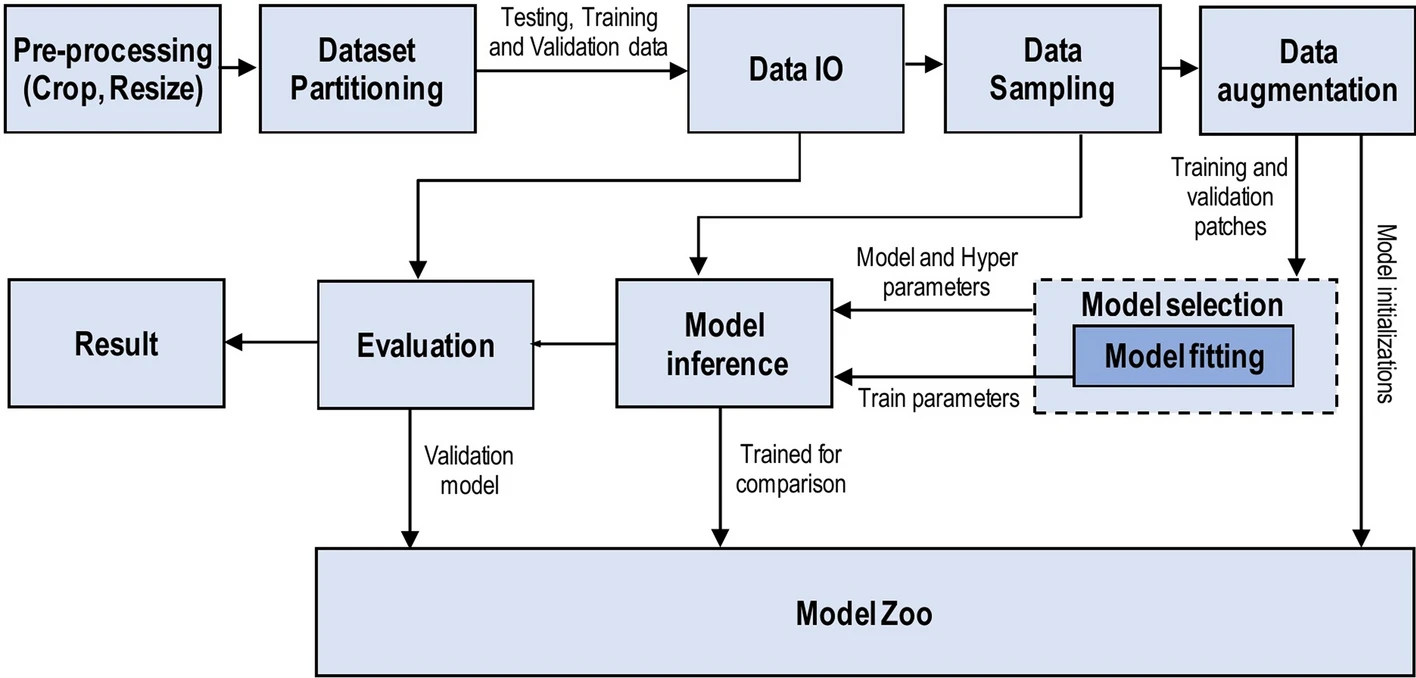
\includegraphics[scale=0.275]{./figures/Pipeline.png}
	\caption{Generic deep learning pipeline}~\label{fig:pipeline}
\end{figure}



\subsubsection{Normalisation of the data}
When working with pre-trained models, normalisation is commonly carried out to adjust for the distribution of the dataset that the model was originally trained on. This can be paired with cropping and resizing the images of the given dataset to fit the dimensions required as input to the pre-trained model. Such normalisation can be related to the first step in the pipeline proposed by Alzubaidini et al., namely  ``Pre-processing (Crop, Resize)'' in Figure~\ref{fig:pipeline}. The normalisation statistics for pre-trained models loaded via PyTorch are generally given as is the case for AlexNet\citep{pytorchAlexNet}. As an implicit hypothesis, the normalisation of the data according to the model that's employed should enable a frictionless usage of said model.


\subsubsection{Balancing of the Dataset}\label{balancingtheory}
As Kaur et al\@.~\citep{kaurbalancing} elucidate in their Systematic Review on Imbalanced Data Challenges
in Machine Learning, an imbalanced dataset can lead to classifications being skewed in favour of the majority class. When working with multi-class classification problems, this applies to the classes with clearly more data points than the other classes. While measures like the Imbalanced Ratio \citep{kulkarni2020foundations} do exist to quantify how unbalanced a dataset is, there commonly doesn't appear to be a strict cut-off value for when a dataset is deemed ``unbalanced''. Nonetheless, it's evident that unbalanced datasets must be dealt with, as Kaur et al\@. describe how the accuracy in these favour the majority class, yielding potentially better accuracy for the majority class while yielding lower accuracy for the minority class. Kulkarni et al\@. also present various methods which essentially rely on oversampling or undersampling classes, sometimes according to some measure \citep{kulkarni2020foundations}. In the generic pipeline for deep learning by Alzubaido et al., Data Sampling can also be found in the early stages of the proposed pipeline, see Figure~\ref{fig:pipeline} PyTorch provides various samplers, among them the WeightedRandomSampler \citep{pytorchTorchutilsdatax2014}, which allows to sample elements according to some given probabilities. In order to balance out a dataset using WeightedRandomSampler provided by PyTorch, the probabilities with which data from a class is drawn needs to be calculated. These probabilities can be determined by dividing 1 by the number of samples in a class. Following this theoretical foundation, the hypothesis is that a balancing of the data improves accuracy as compared to a model which learned on unbalanced data.


\subsubsection{Data Augmentation}\label{augmentationtheory}
Small data size and lack of variation in the data is associated with false predictions and worse accuracy by Maharana et al\@.~\cite{maharana2022review}.  Data quality issues plague many areas of Machine Learning. Maharana et al\@. note that by means of data augmentation, more data can be generated from limited amounts of data and there's also the potential to combat overfitting. Data augmentation is commonly assigned to the data preprocessing part of the deep learning pipeline. Common data augmentation techniques listed by Maharana include: flipping, rotation, noise, shifting, cropping, PCA jittering GAN, and WGAN\@. All these methods listed could, in theory, increase variation in the data and thus avoid overfitting, producing a model more capable of generalisation and capturing a plethora of features instead of being limited to a smaller pool of features of an unaugmented dataset. Considering this, the hypothesis that arises is that data augmentation will help with overall accuracy and overfitting, possibly leading to less false positives and more true positives across for instance a confusion matrix.


\subsubsection{Batch Normalisation}\label{batchnormtheory}
Santurkar et al\@. describe how for Batch Normalisation additional layers are added to the architecture of the network which set the mean and variance of the output to zero and one respectively \citep{santurkar2018does}. In order to retain model expressivity the batch normalised inputs are also shifted and scaled based on trainable parameters. The idea of the Internal Covariate Shift is described by Santurkar et al\@. as one of the reasons batch normalisation was invented. Internal Covariate Shift, it is speculated, essentially is a change of the distribution of inputs to a layer in the network caused by an update of parameters to the previous layers. Furthermore, Internal Covariate Shift is hence presumed to have as a consequence a constant shift of the underlying training problem. However, this remains a controversial concept, as Santurkar et al\@. actually argue that batch normalisation does not reduce Internal Covariate Shift at all. The authors identify the key effect of batch normalisation to be the reparametrisation of the underlying optimisation problem in order to make it more stable. Despite presumably not dealing with the Internal Covariate Shift, batch normalisation thus potentially is a useful addition to a deep learning architecture. Extrapolating from that one arrives at the hypothesis that a network with batch normalisation performs better across given metrics as compared to a network without batch normalisation, ceteris paribus.


\subsubsection{Evaluation Metrics}
Hand et al\@. define various evaluation metrics~\citep{hand2021f} which are commonly found throughout the literature. To facilitate legibility, the following abbreviations are used: total number of positives (P), total number of negatives (N), true positives (TP), true negatives (TN), false positives (FP) and false negatives (FN). A quick definition of these metrics shall be given here as proposed by~\cite{hand2021f}. 

\begin{center}
	Accuracy = $\frac{TP + TN}{P + N}$ \hspace{4em} Precision = $\frac{TP}{TP + FP}$ \hspace{4em} Recall = $\frac{TP}{TP + FN}$ \newline
\end{center}
\begin{center}
	F1-Score = $2 \cdot \frac{Precision \cdot Recall}{Precision + Recall}$
\end{center}